% Manuscript for Bioinformatics Advances (OUP authoring template, texlive-publishers).
% Every number is produced by scripts/paper_numbers.py (DLPFC-specific analyses) and
% scripts/paper_v2.py (all datasets) -> results/paper_numbers*.json, results/table_main.tex.
\documentclass[unnumsec,webpdf,contemporary,large]{oup-authoring-template}
\usepackage{booktabs}
\usepackage{xcolor}
\graphicspath{{../docs/figures/}}
\newcommand{\todo}[1]{\textcolor{red}{[TODO: #1]}}

\journaltitle{Bioinformatics Advances}
\DOI{DOI HERE}
\copyrightyear{2026}
\pubyear{2026}
\access{Advance Access Publication Date: Day Month Year}
\appnotes{Original Paper}
\firstpage{1}

\title[The clustering lottery in spatial domain identification]{The clustering lottery:
initialisation and input-order sensitivity of mixture-model clustering confounds benchmarks of
spatial domain identification}

\author[1,$\ast$]{\todo{First Author}}
\author[1]{\todo{Second Author}}
\authormark{\todo{Author} et al.}
\address[1]{\orgdiv{\todo{Department}}, \orgname{\todo{University}}, \orgaddress{\country{\todo{Country}}}}
\corresp[$\ast$]{Corresponding author. \href{mailto:email@example.org}{\todo{email}}}

\received{Date}{0}{Year}
\revised{Date}{0}{Year}
\accepted{Date}{0}{Year}

\abstract{\textbf{Motivation:} New methods for spatial domain identification are usually
compared by small differences in adjusted Rand index (ARI), mostly on the twelve human DLPFC
Visium sections. Most of them obtain domains by fitting a Gaussian mixture model (typically
mclust, EEE) once to a learned embedding. How much of the reported differences is due to the
encoder and how much to this final clustering step is rarely measured.\\
\textbf{Results:} We evaluated two graph deep-learning methods (HiSTaR, GraphST), BANKSY,
SpaGCN and training-free graph-diffusion baselines on 20 annotated sections from three
technologies (10x Visium, STARmap, MERFISH), with three seeds each. With its official code,
HiSTaR reached a median ARI of 0.51 on DLPFC instead of the reported 0.65. On 60 fixed embeddings, refitting the same mixture model from different random starts changed ARI by
0.17 on average and by up to 0.54; selecting the best of 20 fits by ARI would inflate results by 0.08.
R mclust is deterministic for a given input, but merely permuting the order of the spots changed
its ARI by up to 0.29, and adding noise at 1\% of the feature scale by up to 0.53. Selecting fits
by likelihood did not resolve this: likelihood and ARI were negatively correlated on MERFISH.
Under matched clustering, neither deep model outperformed a training-free linear graph-diffusion
baseline on any of the three datasets, and method rankings changed with the clustering protocol.
We give five reporting recommendations for benchmarks.\\
\textbf{Availability and implementation:} Code, per-run results and figures: \todo{GitHub URL and
Zenodo DOI}. All public data sources are listed in the Data availability section.}

\keywords{spatial transcriptomics, spatial domains, clustering, reproducibility, benchmarking}

\begin{document}
\maketitle

\section{Introduction}

Spatial transcriptomics measures gene expression at thousands of locations in a tissue section
while retaining their coordinates. Identifying \emph{spatial domains}, regions with coherent
expression such as cortical layers, is one of the first analyses of such data, and many methods
have been proposed for it, from Bayesian models \citep{zhao2021bayesspace} and
neighbourhood-augmented features \citep{singhal2024banksy} to graph neural networks
\citep{hu2021spagcn,dong2022stagate,long2023graphst} and hierarchical graph variational
autoencoders such as HiSTaR \citep{yu2025histar}.

Most of these methods are evaluated on the twelve manually annotated human dorsolateral prefrontal
cortex (DLPFC) sections \citep{maynard2021dlpfc} and report median ARI improvements of a few
hundredths over previous methods. Many share the same last step: the learned embedding is clustered
once with mclust's EEE Gaussian mixture \citep{scrucca2016mclust}. Benchmarks have found that
rankings depend strongly on the dataset \citep{yuan2024benchmark,nar2025bench}, that deep methods
vary with the random seed \citep{nar2025bench}, that replacing each method's clustering algorithm
changes results \citep{hu2024gbbench}, and that preprocessing and clustering choices often matter
more than architectural novelty \citep{explanatory2026}. Simple training-free pipelines are also
competitive \citep{nichepca2025,do2026graphbg}.

We complement these studies with a direct measurement of the variance contributed by the
clustering step itself. We ask: (1) do HiSTaR's published DLPFC results reproduce with the
official code; (2) on a \emph{fixed} embedding, how much does ARI change with the initialisation of
the mixture model, and with perturbations that leave the data essentially unchanged (spot order,
negligible noise) under R mclust; (3) does selecting fits by likelihood help; and (4) do encoders
still differ once every embedding is clustered the same way, across three technologies?

\section{Materials and methods}

\subsection{Data}
\textbf{DLPFC (10x Visium).} Twelve sections from three donors \citep{maynard2021dlpfc}; seven
annotated layers (five for donor 2), \texttt{layer\_guess\_reordered}.
\textbf{STARmap mouse medial prefrontal cortex.} Three sections (about 1050 cells, 166 genes) with
four annotated layers (L1, L2/3, L5, L6) \citep{wang2018starmap}.
\textbf{MERFISH mouse hypothalamus.} Animal 1, five sections from Bregma $-0.04$ to $-0.24$ (about
5500 cells, 155 genes) with eight annotated regions \citep{moffitt2018merfish}. The STARmap and
MERFISH annotations are those distributed with the BASS analyses \citep{li2022bass}. In total, 20
sections from three technologies.

\subsection{Preprocessing}
DLPFC: genes in fewer than 50 spots or with fewer than 10 counts were removed, 2000 highly
variable genes were selected (Seurat v3 flavour), counts were library-size normalised,
log-transformed and scaled, and reduced to 200 principal components (PCs). STARmap and MERFISH
(targeted panels): all genes, same normalisation, 50 PCs. All methods received the same input
where they accept one; BANKSY used the log-normalised genes and SpaGCN and GraphST their own
documented preprocessing. The true number of domains was given to every method, and unannotated
spots were excluded from evaluation.

\subsection{Methods}
\begin{itemize}
\item \textbf{HiSTaR} \citep{yu2025histar}: PyTorch port of the official code with the published
defaults (cross-level weight 0.3, 200+200 epochs).
\item \textbf{GraphST} \citep{long2023graphst}: official package and tutorial pipeline
(600 epochs, 20-PC embedding, R mclust EEE; with and without its label refinement). Because of its
CPU cost, GraphST was run with one seed on DLPFC and three seeds on STARmap and MERFISH.
\item \textbf{BANKSY} \citep{singhal2024banksy}: official \texttt{pybanksy}, 18 neighbours,
$m_{\max}=1$, $\lambda\in\{0.2,0.8\}$, 20 PCs.
\item \textbf{SpaGCN} \citep{hu2021spagcn}: official tutorial pipeline without histology
($p=0.5$, Louvain resolution search to the true number of domains, 200 epochs).
\item \textbf{Training-free baselines.} \emph{Linear diffusion}: the top 30 PCs are smoothed on the
spatial 6-nearest-neighbour graph, $H^{(t+1)}=(1-\alpha)H^{(t)}+\alpha D^{-1}AH^{(t)}$,
$\alpha=0.5$, $T=10$. \emph{AnisoST}: the same with edge weights recomputed at every step,
$w_{ij}^{(t)}=\exp(-\|h_i^{(t)}-h_j^{(t)}\|^2/\kappa^{(t)})$ (Perona--Malik-type edge-preserving
diffusion \citep{perona1990}; $\kappa^{(t)}$ the median squared edge difference); a similar idea has
been used inside a deep model \citep{wang2024pearlst}. \emph{PCA} without smoothing is the
non-spatial reference. All baseline settings were fixed on DLPFC donor 1 before any other data
were analysed, and none were tuned on STARmap or MERFISH.
\end{itemize}

\subsection{Clustering protocols}
All embeddings except SpaGCN's (which clusters internally) were clustered with a tied-covariance
Gaussian mixture, the mclust EEE model. \emph{Standard}: each method's usual call, i.e.\ R mclust
for GraphST and a 3-start scikit-learn GMM \citep{pedregosa2011sklearn} with a fixed seed for the
others. \emph{Robust}: 20 random starts, keeping the fit with the highest log-likelihood (label
free). \emph{Lottery}: one seed-0 embedding per section and method, clustered 20 times with a
single random start each. \emph{mclust perturbations}: R mclust (version 6.0.1, default
hierarchical initialisation) on the same embedding (i) unchanged, (ii) after random permutation of
the rows, 10 times, and (iii) after adding Gaussian noise with 1\% of each feature's standard
deviation, 10 times.

\subsection{Evaluation and statistics}
ARI \citep{hubert1985ari} against the manual annotation; NMI gave the same conclusions (code
repository). For every (method, section) we average over seeds. Methods were compared with
two-sided Wilcoxon signed-rank tests over sections, with Holm correction \citep{holm1979} within
each family of comparisons. Runtimes are single-thread CPU wall-clock times.

\section{Results}

\subsection{HiSTaR's published DLPFC results did not reproduce}
With the official code and defaults, HiSTaR reached a median ARI over the twelve DLPFC sections of
0.509 (mean 0.491, 95\% bootstrap CI 0.454--0.525) with the 3-start GMM, and 0.449 (mean, seed 0)
when its embedding was clustered with R mclust as in the official pipeline, compared with a reported
median of 0.65 \todo{verify the reported values (0.65 median; 0.718 on 151673) against the HiSTaR
article}. Fixing a bug that applies random masking at inference did not change accuracy (0.487).
Possible causes include per-section tuning of the loss weights (described in the HiSTaR supplement),
unpublished preprocessing and the choice of seed; the following sections show that the clustering
step alone produces differences of this size. \todo{Report the outcome of contacting the authors.}

\subsection{On a fixed embedding, the clustering step alone moves ARI by up to 0.54}
Figure~\ref{fig:lottery} shows the ARI of 20 single-start fits of the same mixture model on each
fixed embedding. Across the 60 HiSTaR, GraphST and AnisoST embeddings, the ARI range within an
embedding was 0.17 on average and reached 0.54 (HiSTaR, STARmap). The size of the effect depended
on the embedding: average ranges were 0.21--0.23 for HiSTaR and AnisoST on DLPFC, 0.25--0.41 on
STARmap and 0.11--0.15 on MERFISH, whereas GraphST's 20-dimensional PCA embeddings were more stable
(0.13 on DLPFC, 0.06 on STARmap, 0.03 on MERFISH). The best of the 20 fits by ARI exceeded the
average single fit by 0.08: choosing a clustering run by its agreement with the labels, explicitly
or by trying a few seeds, would inflate a reported result by about as much as the gap between most
published methods.

\begin{figure*}[t]
\centering
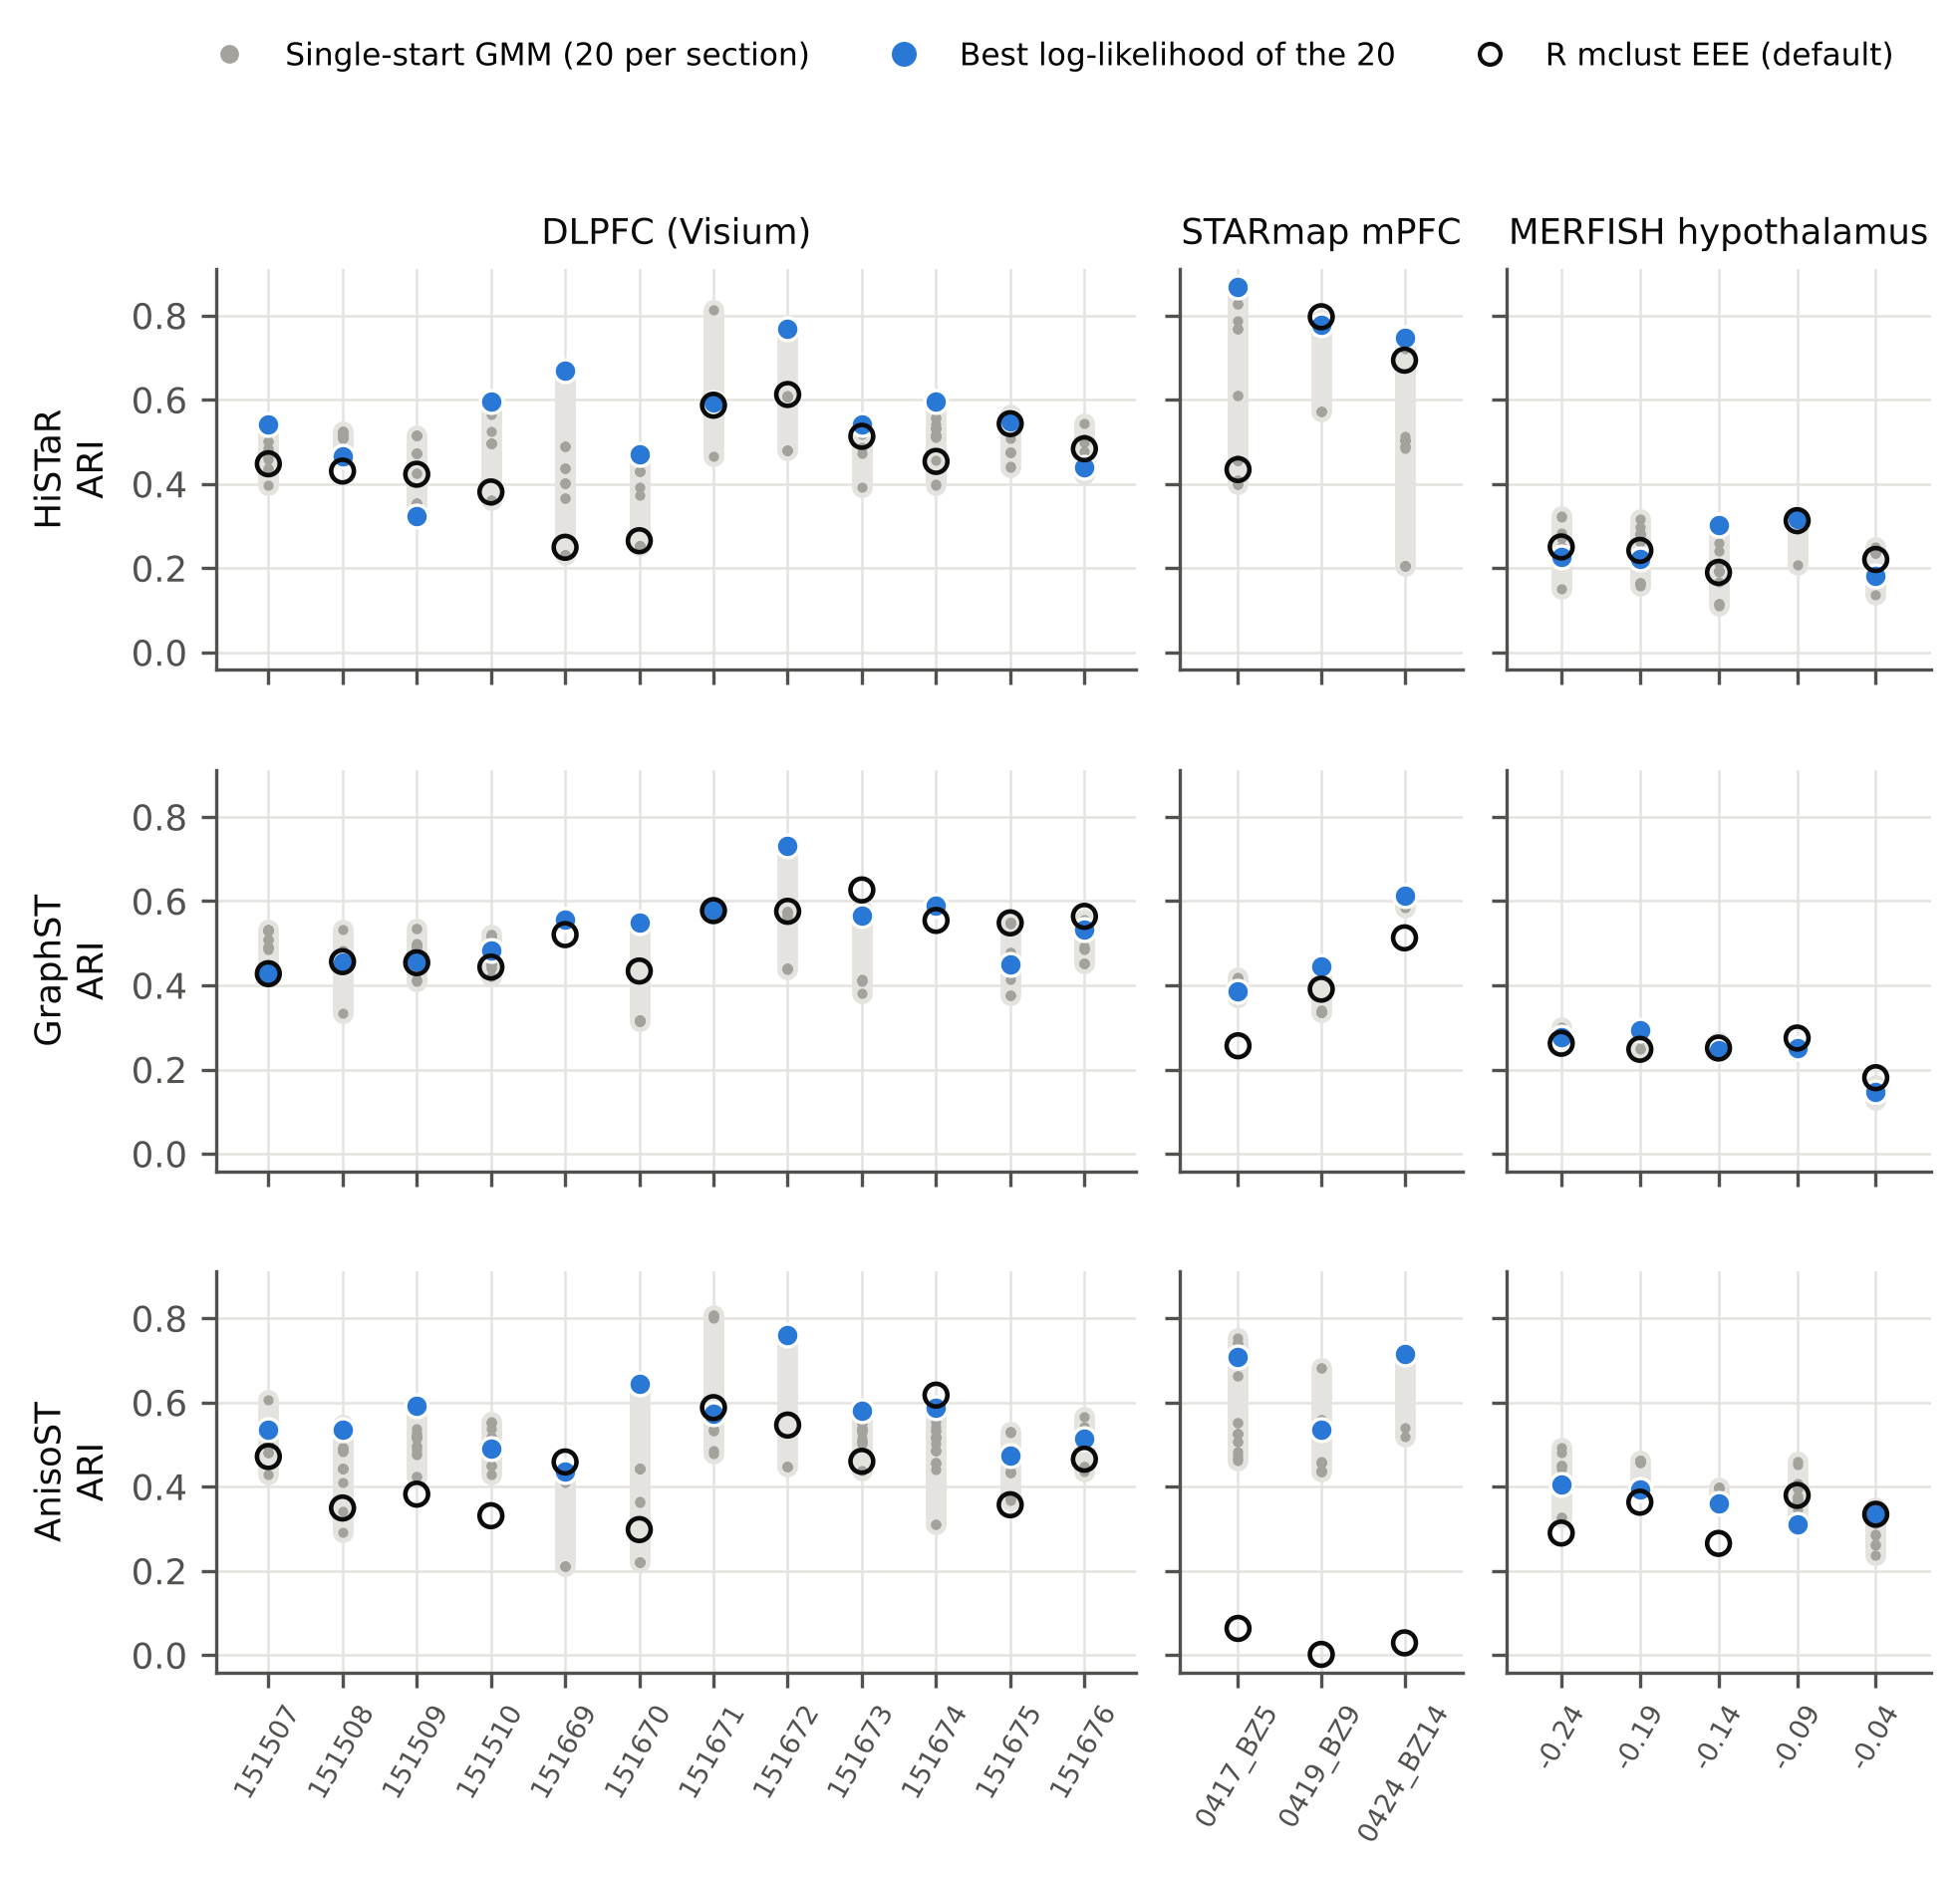
\includegraphics[width=\linewidth]{v2_fig1_lottery.png}
\caption{The clustering lottery. For each section, one fixed embedding was clustered 20 times with a
single-start tied-covariance GMM (grey dots; bar = range). Blue: the fit with the highest
log-likelihood (label-free). Open circle: R mclust with default settings on the same embedding.}
\label{fig:lottery}
\end{figure*}

\subsection{R mclust is deterministic but not stable}
mclust initialises EM by model-based hierarchical agglomeration, so one call on a fixed embedding
always returns the same partition. That partition, however, depended on details that carry no
information (Fig.~\ref{fig:mclust}). Randomly permuting the order of the spots changed ARI by
0.11--0.14 on average within an embedding on DLPFC (up to 0.29) and by 0.09--0.14 on MERFISH; on DLPFC, 22--43\% of the permutations moved ARI by more than 0.05 for HiSTaR and AnisoST, and
11\% for GraphST. Adding noise at 1\% of each
feature's standard deviation had similar effects, and on STARmap changed the ARI of HiSTaR
embeddings by 0.39 on average (up to 0.53). On all three STARmap sections mclust's default fit was
degenerate for the AnisoST embedding, with one cluster holding about 95\% of the cells and the
others only 8--31 cells each (ARI 0.00--0.06), a failure the random-start fits did not show. Over all 60 embeddings, mclust's default fit had
a lower mean ARI (0.40) than the best-likelihood fit of 20 random starts (0.50) and reached a
log-likelihood at least as high in only 42\% of cases.

\begin{figure*}[t]
\centering
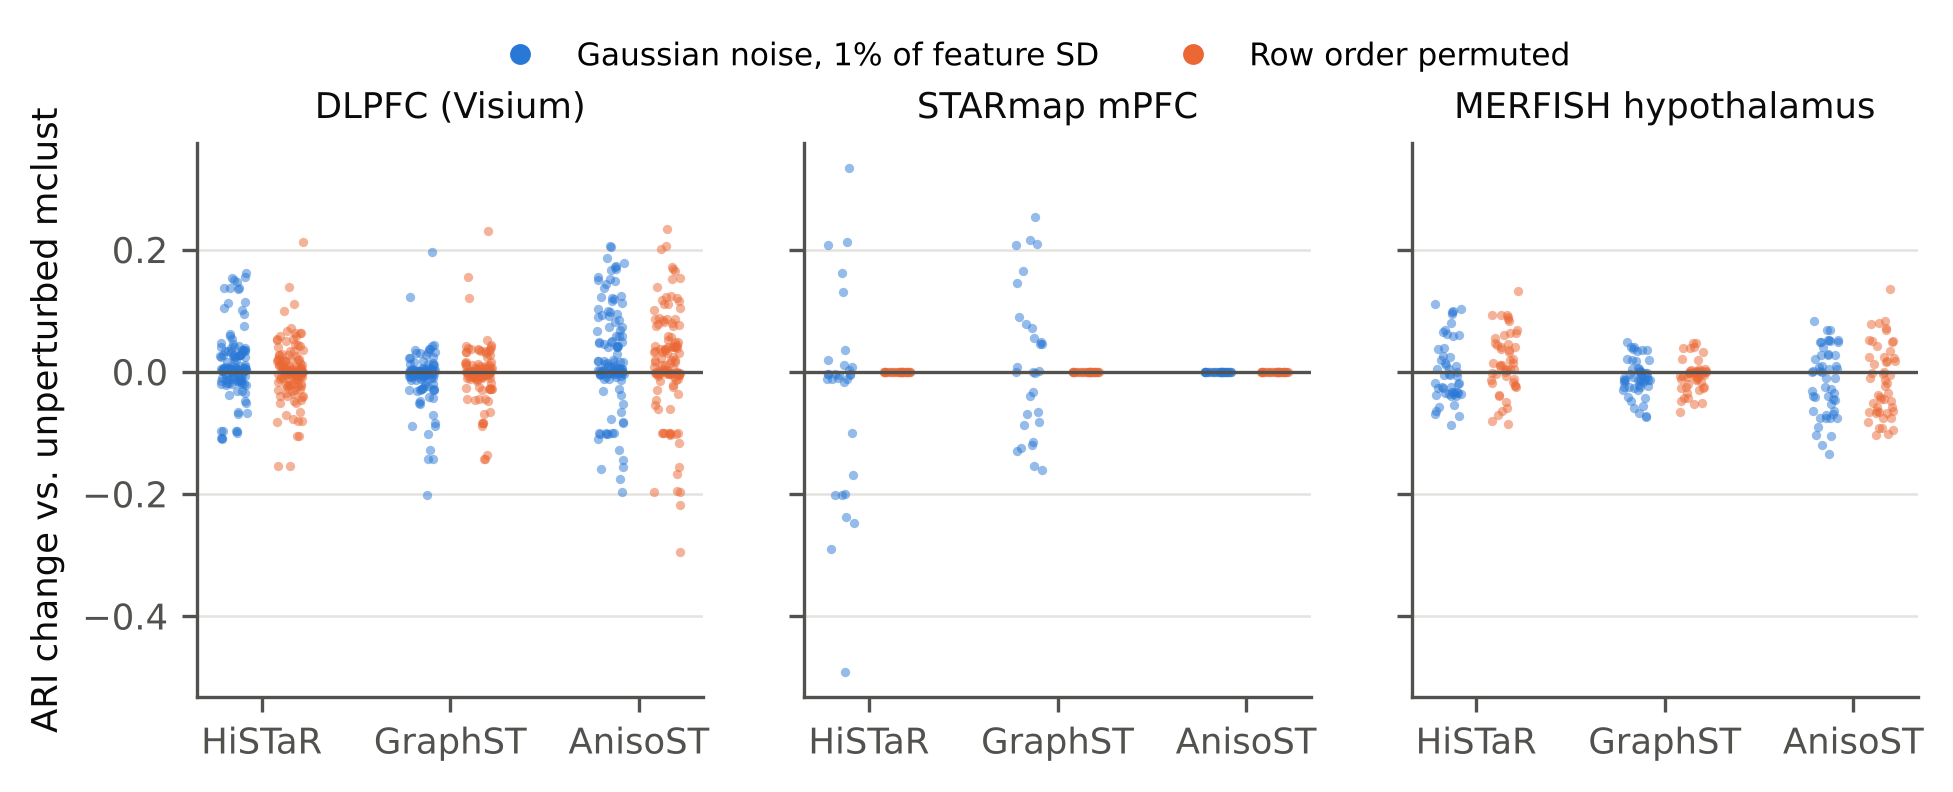
\includegraphics[width=0.85\linewidth]{v2_fig2_mclust.png}
\caption{Change in ARI of R mclust (EEE, default initialisation) when the same embedding is
perturbed by permuting the spot order (orange) or adding noise at 1\% of each feature's standard
deviation (blue); 10 perturbations per section and embedding.}
\label{fig:mclust}
\end{figure*}

\subsection{Choosing fits by likelihood is not a remedy}
A natural fix is to run many starts and keep the most likely fit. It helped some embeddings and
not others. Across all 20 sections, it raised HiSTaR's mean ARI by 0.053 (14/20 sections,
$p=0.004$) and GraphST's by 0.025 (13/20, $p=0.11$), and did not change BANKSY $\lambda=0.8$
(+0.003, 9/20, $p=0.68$; negative on STARmap and MERFISH). The reason is visible in Fig.~\ref{fig:lottery}: likelihood and ARI were positively
related on DLPFC and STARmap (median Spearman $\rho$ 0.22--0.53) but negatively on MERFISH
($-0.36$ to $-0.57$), where the best-fitting mixture separates cell types rather than anatomical
regions. Better optimisation of the mixture model is therefore not the same as better domains.

\subsection{Under matched clustering, deep encoders did not outperform a training-free baseline}
Table~\ref{tab:main} and Fig.~\ref{fig:matched} compare all methods under both protocols.
Linear graph diffusion had the highest or near-highest mean ARI on all three datasets (DLPFC
0.558, STARmap 0.705, MERFISH 0.497). Over the 20 sections it outperformed HiSTaR with standard
clustering (+0.126, 17/20 sections, Holm-adjusted $p=0.005$), GraphST with its own mclust clustering (+0.135, 14/20, adjusted $p=0.016$) and with robust
clustering (+0.110, 16/20, adjusted $p=0.016$), and SpaGCN (+0.234, 20/20, $p<0.001$). Even with its
label refinement, GraphST did not reach linear diffusion on any dataset (DLPFC 0.548, STARmap
0.550, MERFISH 0.366). Differences to HiSTaR with robust
clustering (+0.074, 14/20, adjusted $p=0.069$) and to BANKSY $\lambda=0.8$ (+0.048 to +0.051,
adjusted $p=0.069$) were not significant after correction. The ranking of the deep methods relative
to the baselines changed with the clustering protocol (Fig.~\ref{fig:matched}). The deep methods
were also the least stable: HiSTaR's seed-to-seed standard deviation of ARI was 0.047 on DLPFC and
0.18 on STARmap, against 0.003--0.04 for the training-free baselines, and they were the slowest
(median 23~min per DLPFC section for GraphST and 1--2~min for HiSTaR on one CPU thread, against
3~s for linear diffusion).

\begin{table*}[t]
\centering
\caption{Mean ARI over sections (3 seeds per section; GraphST on DLPFC: 1 seed). Standard: each
method's usual clustering (R mclust for GraphST; 3-start GMM otherwise; SpaGCN clusters
internally). Robust: 20-start GMM, best likelihood. $^\dagger$Training-free; all baseline settings
fixed on DLPFC donor 1.}
\label{tab:main}
\begin{tabular}{lcccccc}
\toprule
 & \multicolumn{2}{c}{DLPFC (Visium)} & \multicolumn{2}{c}{STARmap mPFC} & \multicolumn{2}{c}{MERFISH hypothalamus} \\
 & Standard & Robust & Standard & Robust & Standard & Robust \\
\midrule
Linear diffusion$^\dagger$ & -- & 0.558 & -- & 0.705 & -- & 0.497 \\
AnisoST$^\dagger$ & 0.526 & 0.551 & 0.564 & 0.622 & 0.377 & 0.363 \\
PCA, non-spatial$^\dagger$ & -- & 0.409 & -- & 0.294 & -- & 0.130 \\
BANKSY $\lambda=0.8$ & 0.494 & 0.518 & 0.740 & 0.694 & 0.428 & 0.410 \\
BANKSY $\lambda=0.2$ & 0.514 & 0.518 & 0.502 & 0.529 & 0.211 & 0.222 \\
HiSTaR & 0.491 & 0.544 & 0.593 & 0.658 & 0.221 & 0.264 \\
GraphST & -- & -- & 0.388 & 0.484 & 0.251 & 0.254 \\
SpaGCN & 0.422 & -- & 0.267 & -- & 0.151 & -- \\
\bottomrule
\end{tabular}

\end{table*}

\begin{figure*}[t]
\centering
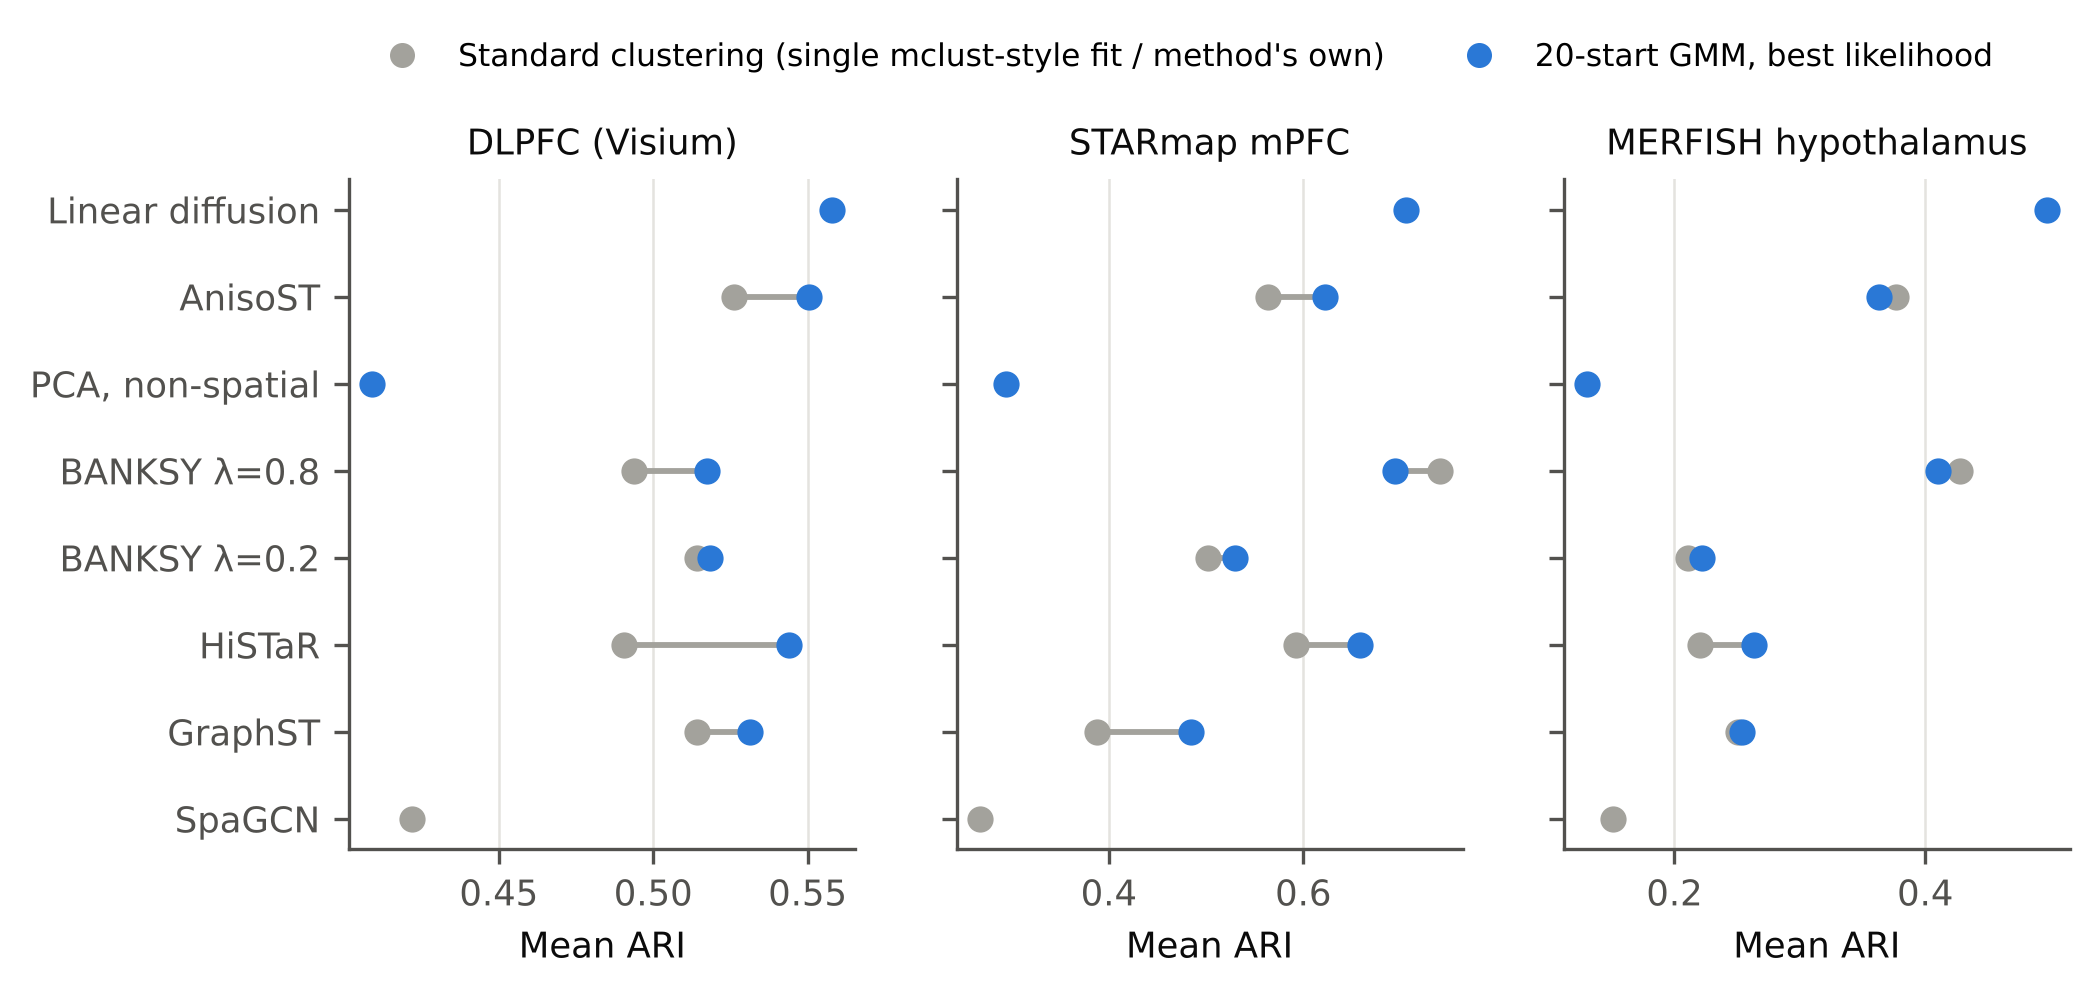
\includegraphics[width=\linewidth]{v2_fig3_matched.png}
\caption{Mean ARI per dataset with standard clustering (grey) and the 20-start, best-likelihood GMM
(blue) applied to the same embeddings.}
\label{fig:matched}
\end{figure*}

\subsection{Edge preservation helps at boundaries on Visium but not on single-cell data}
On DLPFC, AnisoST matched linear diffusion in ARI (0.551 vs 0.558) and improved accuracy on spots
at layer boundaries by 0.025 (9/12 sections, $p=0.034$, uncorrected) without changing interior
accuracy (Supplementary Fig.~S2). On MERFISH it was clearly worse (0.363 vs 0.497): at single-cell
resolution neighbouring cells often differ by cell type, so an edge-preserving rule blocks the
smoothing that is needed to reveal regions. We report this as a negative result for the
edge-preserving variant; the simpler linear diffusion was the more robust baseline.

\section{Discussion}
The final clustering step of spatial domain methods is a substantial and under-reported source of
variance. On fixed embeddings from three technologies, random initialisation alone spanned 0.17 ARI on average, and the R implementation used by most published methods changed its answer when the
spots were merely reordered. Better likelihood did not reliably mean better domains, and under
matched clustering a training-free diffusion baseline was not outperformed by the deep encoders we
tested. These results agree with recent large benchmarks
\citep{explanatory2026,hu2024gbbench,nar2025bench} and add a direct, quantitative measurement of
clustering variance on fixed embeddings.

\paragraph{Recommendations.} (1) Report the clustering protocol: algorithm, implementation and
version, initialisation, number of starts, seeds, and how they were chosen. (2) Never select seeds
or runs by agreement with the labels. (3) Report distributions over training seeds \emph{and}
clustering runs (or input permutations), with per-section values. (4) Compare encoders under the
same clustering, and include training-free baselines such as neighbourhood smoothing. (5) Report
runtime and seed variance alongside accuracy.

\paragraph{Limitations.} We tested two deep encoders, BANKSY and SpaGCN; STAGATE, SEDR, BayesSpace and
other methods were not included. GraphST was run with one seed on DLPFC. The STARmap and MERFISH
annotations are coarse and the STARmap data contain only three small sections. The number of domains
was given to every method. We could not reproduce HiSTaR's per-section tuning. The lottery
experiments use one embedding per section and method; training-seed variance is reported separately.

\section*{Competing interests}
No competing interest is declared.

\section*{Author contributions statement}
\todo{CRediT statement.}

\section*{Use of AI tools}
\todo{Describe per journal policy: code, experiments and a first draft of this manuscript were
produced with the assistance of an AI coding assistant (Claude, Anthropic); all results were
checked by the authors, who take full responsibility for the content.}

\section*{Data availability}
DLPFC: spatialLIBD (count matrices) and SEDR analyses repository (layer annotations). STARmap and
MERFISH with domain annotations: BASS-Analysis repository \citep{li2022bass}, from the original
studies \citep{wang2018starmap,moffitt2018merfish}. Scripts that download and convert all data are
provided with the code.

\section*{Funding}
\todo{Funding.}

\bibliographystyle{abbrvnat}
\bibliography{refs}

\clearpage
\section{Supplementary figures}
\renewcommand{\thefigure}{S\arabic{figure}}
\setcounter{figure}{0}

\begin{figure*}[h]
\centering
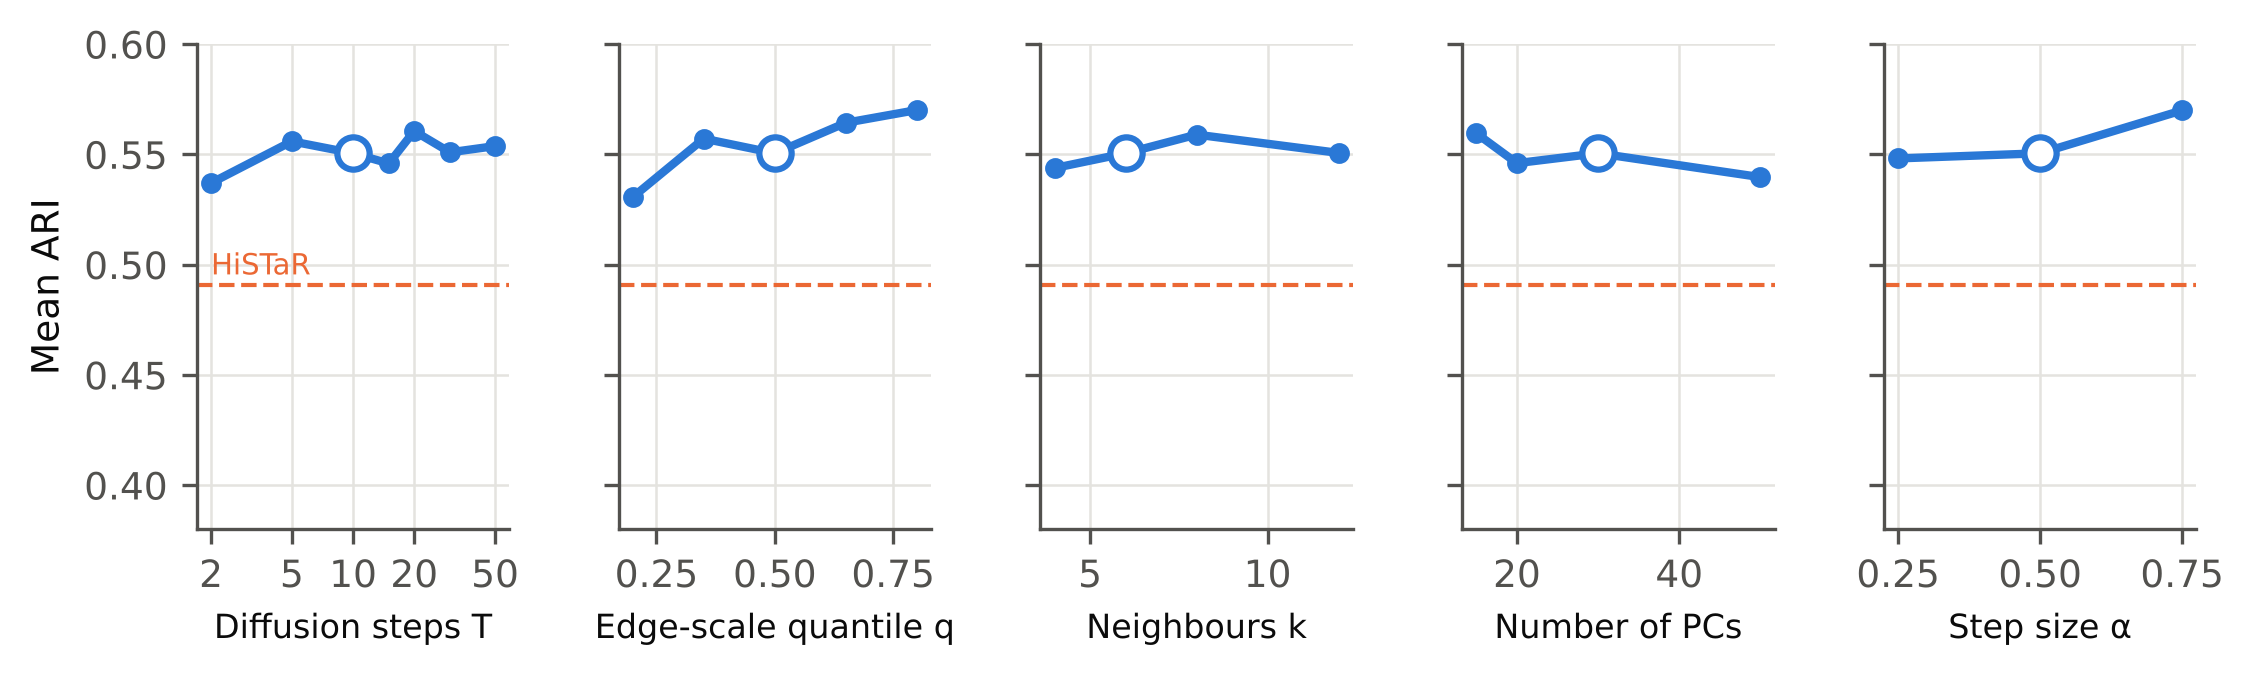
\includegraphics[width=0.9\linewidth]{fig3_sensitivity.png}
\caption{DLPFC: mean ARI of AnisoST when one hyper-parameter is changed at a time; open circle =
default; dashed = HiSTaR, standard clustering.}
\end{figure*}

\begin{figure}[h]
\centering
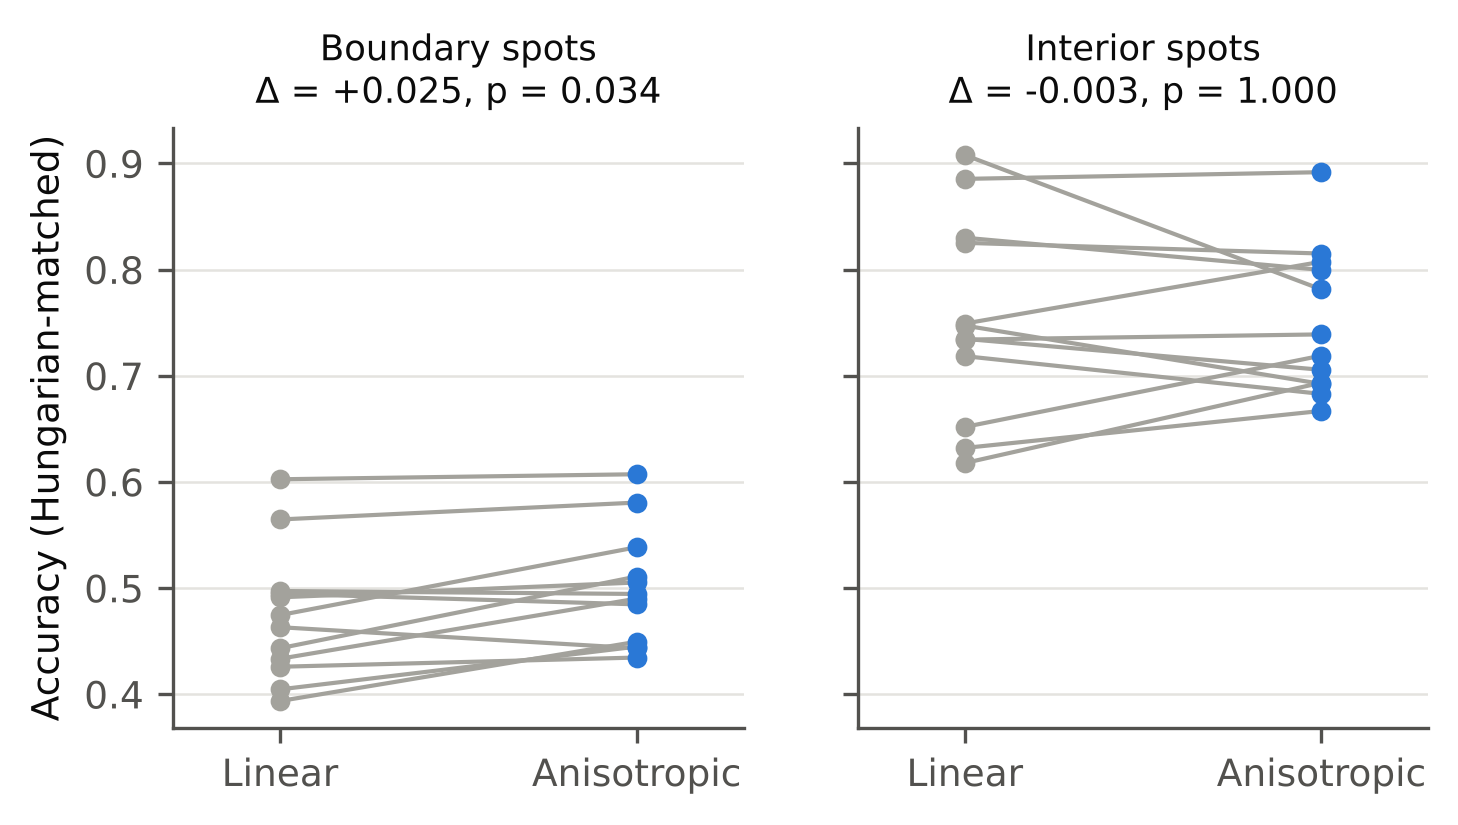
\includegraphics[width=\linewidth]{fig4_boundary.png}
\caption{DLPFC: accuracy on boundary and interior spots, linear vs.\ edge-preserving diffusion; one
line per section.}
\end{figure}

\begin{figure*}[h]
\centering
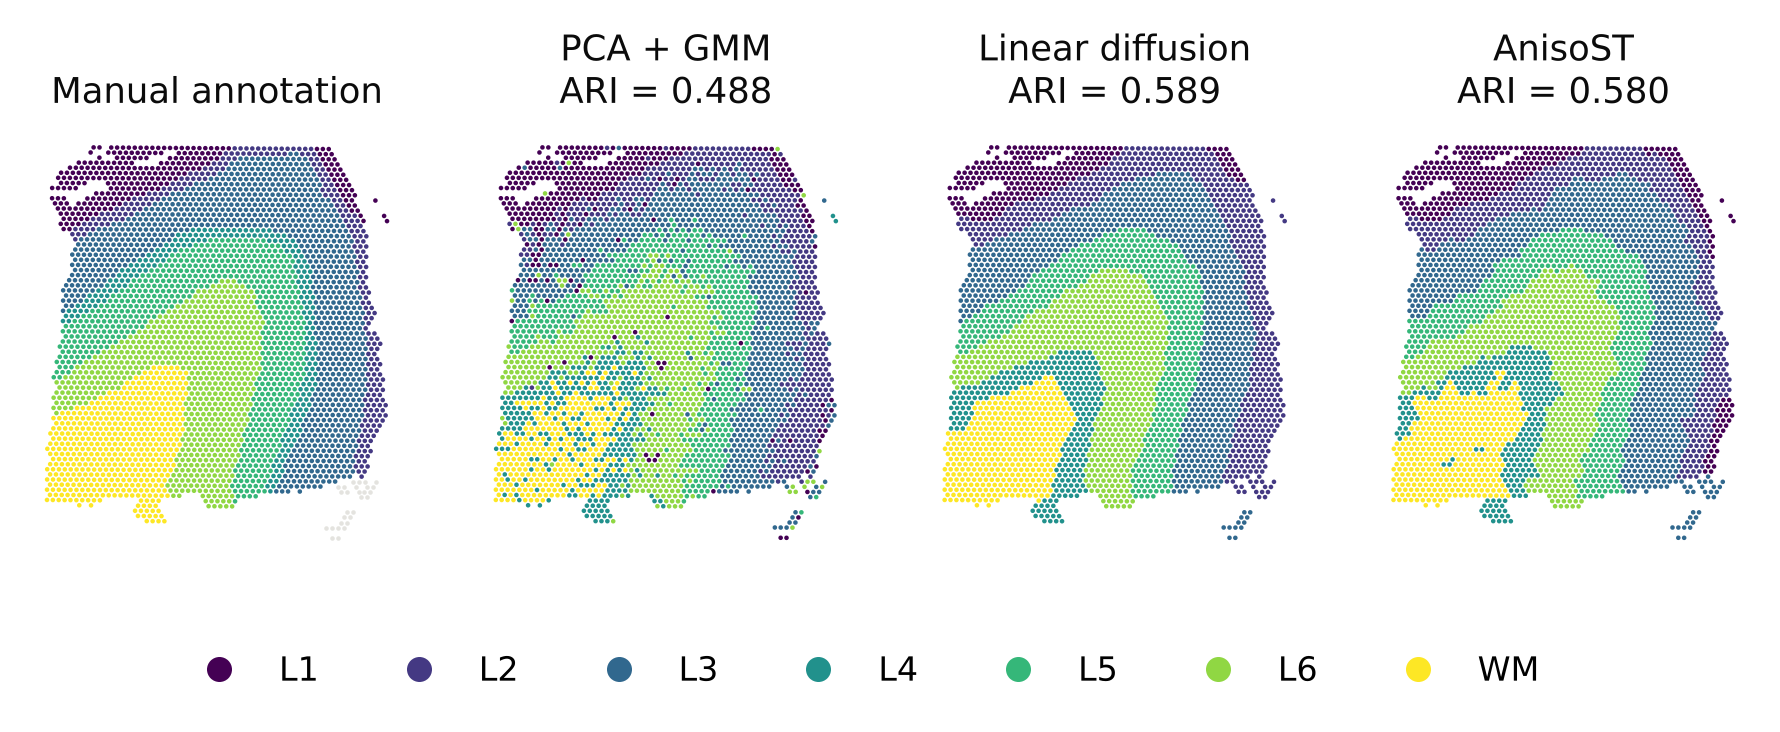
\includegraphics[width=\linewidth]{fig5_spatial_151673.png}
\caption{DLPFC section 151673: manual annotation and domains from PCA + GMM, linear diffusion and
AnisoST.}
\end{figure*}

\end{document}
